\chapter{Design}
\label{Chapter4}
\lhead{Chapter 4. \emph{Design}} 

This section gives an overview of the design of our RPC framework and generator. The main design decisions were regarding three different issues. These are

\begin{itemize}
	\item The overall RPC framework structure. This refers to how the RPC framework is split up into different layers, and the design issues of each layer.
	\item WebIDL bindings, and the issues involved with implementing reasonable bindings for JavaScript and C++.
	\item Generating RPC code using WebIDL.
\end{itemize}

\section{RPC Framework} % (fold)
\label{sec:rpc_framework_structure}

The structure of the RPC framework is based around the notion of layers. 
Each layer solves a particular task, in order to achieve the goal of getting from a JavaScript stub to a C++ function, and back. Listing \ref{structurediagram} shows the overall structure and interactions of each layer.

The advantages of this approach is that each layer is independent of the other. For example, if we choose a different RPC schema (i.e. something other than JSON RPC), we could easily replace the JSON RPC layer. Or, if we choose to have the C++ function on the server instead of as a Native Client module, we can easily change the transport layer to use AJAX requests or Web Sockets. 


The other advantage to this approach is that because the layers are independent and each layer has a simple interface, each layer can easily be tested. For example, to test the implementation of the run time layer, we can easily mock the JSON RPC layer, since we know its public interface.

In the end, we have four layers: the stub layer, runtime layer, JSON RPC layer and transport layer. Each layer is described in detail below.

\lstset{language=c,caption={A layered approach to RPC},label=structurediagram}
\begin{code}
TODO: Turn it into a real diagram.
+-------------------------------------------------------------------+
|                           NaClRPCModule                           |
|-------------------------------------------------------------------|
|                                                                   |
|                                                                   |
|     +-------------------------------------------------------+     |
|     |+-----------------------------------------------------+|     |
|     || +--------------------+ Stub +----------------------+|| 1   |
|     |+-----------------------------------------------------+|     |
|     +-------------------------------------------------------+     |
|                 +                      ^            ^             |
|                 |                      |            |             |
|                 |callRPC               |successCB   |errorCB      |
|                 |                      |            |             |
|                 v                      +            +             |
|     +-------------------------------------------------------+     |
|     |                        Runtime                        | 2   |
|     +-------------------------------------------------------+     |
|      +          +        +                ^           ^           |
|      |          |        |                |handle     |           |
|      |send      |send    |send            |Callback   |handle     |
|      |Callback  |Error   |Request         |/handleCall|Error      |
|      v          v        v                +           +           |
|     +-------------------------------------------------------+     |
|     |                        JSONRPC                        | 3   |
|     +-------------------------------------------------------+     |
|      +         +         +                ^                       |
|      |         |         |                |                       |
|      |sendRPC  |sendRPC  |sendRPC         |handleRPCCallback      |
|      |Callback |Error    |Request         |/ handleRPCCall        |
|      v         v         v                +                       |
|     +-------------------------------------------------------+     |
|     |                       Transport                       | 4   |
|     +-------------------------------------------------------+     |
|         +        +       +                ^                       |
|         |        |       |                |                       |
|         |        |       |                |                       |
|         |on      |load   |postMessage     |handleMessage          |
|         |        |       |                |                       |
|         v        v       v                +                       |
|     +-------------------------------------------------------+     |
|     |+-----------------------------------------------------+|     |
|     ||+-------------------+ NaClModule +------------------+|| 5   |
|     |+-----------------------------------------------------+|     |
|     +-------------------------------------------------------+     |
|                                                                   |
+-------------------------------------------------------------------+
\end{code}


\subsection{Transport layer} % (fold)
\label{sub:transport_layer_design}
The role of the transport layer is to implement the transportation of messages. Messages could be anything, JavaScript objects, strings, or even binary data. Moreover, the receiver could be anything - a node.js server, or a Native Client module. Finally, the transport could use any transport mechanism - web sockets, HTTP/AJAX, WebRTC, postMessage, etc.

The important thing is that the transport must provide:
\begin{itemize}
	\item An asynchronous API (should be non-blocking)
	\item The following public API:
	\begin{itemize}
		\item a \lstinline+send+ function, that accepts a payload of any type.
		\item a constructor which sets a message handler.
		\item the message handler must be invoked when a message is received. 
	\end{itemize}
\end{itemize}

The reason this approach was taken was to allow any possibility of executing remote procedure calls. It also allows the transport layer to be testable, since no concrete implementations of the layers above or below the transport layer need to be provided to test the functionality of the transport layer.


\subsubsection{Implementing the Transport Layer in JavaScript} % (fold)
\label{ssub:implementing_the_transport_layer_in_javascript}
To implement the transport layer using a Native Client module, we first encapsulate the details of a Native Client module into its own class, called \lstinline{NaClModule}. This class essentially does all the DOM manipulation for a module. To explain this, consider how a Native Client module is normally embedded in the page (as described in the background section \ref{sub:nacl_modules_ppapi} on page \pageref{sub:nacl_modules_ppapi}). The module is embedded onto the page using an \lstinline{embed} tag. The \lstinline{src} attribute points to the location of the NaCl Manifest - which tells the browser which (p)nacl executable to load. For example, \lstinline{<embed src="myModule.nmf" type="application/x-nacl" />}. The \lstinline{type} attribute tells the browser what MIME type the executable is. This could take values of either \lstinline{x-nacl} for NaCl modules or \lstinline{x-pnacl} for PNaCl modules. 

All this detail is configured through the NaClModule constructor, which takes in an object for configuration. In other words, the same \lstinline{embed} tag is created (but not actually placed on the page \emph{yet}), using the following code:

\begin{code}
var myModule = new NaClModule({
  src: 'rpc-module.nmf', 
  name: 'rpc', 
  id: testModuleId, 
  type: 'application/x-pnacl'
});
\end{code}

However, much of the details of this can be `inferred' using the name of the module:

\begin{code}
var myModule = new NaClModule({"name": testModuleId});
// creates an embed tag with the same attributes
\end{code}

The attributes are inferred by using the NaClConfig global object, or a default config object if one does not exist. TODO: Examples of attribute inference using config.

Once a NaClModule is constructed, it can be loaded using the \lstinline{load} method, which can take in an optional callback function as a parameter. The load method essentially inserts the \lstinline{embed} element into the page. Event handlers can be registered with the module by using the \lstinline{on} method. For example:

\begin{code}
var myModule = new NaClModule({"name": testModuleId});
myModule.on('load', function(){...});
myModule.on('message', function(){...});
myModule.on('crash', function(){...});
...
\end{code}

TODO: Class diagram showing NaClModule and Transport.

The NaClModule class therefore makes it easy to create and alter the HTML embed tag using only JavaScript. 

Now, the transport layer encapsulate a NaClModule object, which is used as a low-level communication object in order to send and receive messages. 
% subsubsection implementing_the_transport_layer_in_javascript (end)

\subsubsection{Implementing the Transport Layer in C++} % (fold)
\label{ssub:implementing_the_transport_layer_in_cpp_}
Since the C++ module is a singleton, the structure of the transport in C++ is a lot simpler. Essentially, the transport is a class that extends the \lstinline{pp::Instance} class provided by the PPAPI, which we use to send and receive messages using \lstinline{pp::Instance::PostMessage} and \lstinline{pp::Instance::HandleMessage}. These methods are overridden in order to link the transport with the layer above.

TODO: Class diagram showing Transport extending pp::Instance.


% subsubsection implementing_the_transport_layer_in_cpp_ (end)

% subsection transport_layer_design (end)

\subsection{RPC layer} % (fold)
\label{sub:json_rpc_layer_design}
The RPC Layer is responsible for validating messages sent and received by the transport. 

Messages \emph{received} by the transport could either be RPC \emph{requests}, \emph{responses}, or \emph{errors}. If a message is one of these three, it should forward the message to the layer above (the \emph{runtime}). If a message is not one of these three possibilities, the message should be ignored as it is not a RPC message.

TODO: Diagram showing flow of messages handled and how they are filtered using the RPC Layer.

The RPC layer can also provide RPC \emph{send} functions, that allow messages to be sent to the layer below. It allows RPC requests, responses and errors to be sent.

TODO: Diagram showing flow of messages sent and how they are filtered using the RPC Layer.

Therefore, the RPC layer has the following API:
\begin{itemize}
	\item a \lstinline+handleMessage+ function, which accepts a payload and is called by the Transport layer when a message is received. \lstinline+handleMessage+ should filter through the messages received to categorise them as requests, responses or errors. Depending on which type of message it is, the layer can call different methods of the layer above.
	\item a \lstinline+sendRequest+ function, which validates messages to be sent as requests, and forwards it down to the transport layer to be sent.
	\item a \lstinline+sendResponse+ function, which validates messages to be sent as responses, and forwards it down to the transport layer to be sent.
	\item a \lstinline+sendError+ function, which validates messages to be sent as errors, and forwards it down to the transport layer to be sent.
\end{itemize}

\subsubsection{Choosing a protocol} % (fold)
\label{ssub:choosing_a_protocol}
We decide to use the JSON RPC 2.0 protocol. TODO: reasons + alternatives.
% subsubsection choosing_a_protocol (end)

\subsubsection{Implementing the JSON RPC Layer} % (fold)
\label{ssub:implementing_the_jsonrpc_layer}
To implement the API discussed above for JSON RPC, we first need to implement validators for messages. These determine what kind of message it is - request, response, error, or none. This is done on both the JavaScript and C++ implementations, as both will have to use the protocol. Then, when a message is received, the layer simply uses these validators to check what kind of message it is. At the same time, it extracts the relevant information about the message. For example, if it is a request, it extracts the method name, parameters, etc. 

To implement the JSON RPC protocol validators, we adhere closely to the specification. Detailed unit tests are written, including passing and failing cases. The validator is then written. This is done for both the C++ and JavaScript implementations.

As well as this, some helper functions were written to create valid RPC requests, responses, and errors.

TODO: Class diagrams showing public API.

On the C++ side, a RPCRequest object is created. The RPCRequest object encapsulates generic (i.e. not necessarily JSONRPC specific) information about a RPC call. This is passed by reference to the layers that need it, so that the validation and extraction only happens once.

TODO: Show how RPCRequest is used between layers, instead of generic `message' objects.

% subsubsection implementing_the_jsonrpc_layer (end)

% subsection json_rpc_layer_design (end)

\subsection{RPC Runtime layer} % (fold)
\label{sub:rpc_runtime_layer_design}
The main job of the runtime layer is to coordinate RPC requests and responses. As described in the background section \ref{sub:rpcruntime_background} (page \pageref{sub:rpcruntime_background}), the runtime does this by keeping track of RPC requests, and matching the requests with the responses by the use of a call identifier.

The API the runtime provides is therefore as follows:
\begin{itemize}
	\item send functions, that call the layer below.
	\begin{itemize}
		\item \lstinline+sendRequest = function(method, parameters, successCB, errorCB)+ this will give the request an ID, then keep track of that ID and the callback functions.
		\item \lstinline+sendResponse = function(id, result)+ this will just construct a response message and send it to the layer below.
		\item \lstinline+sendError = function(id, errorCode, errorMessage, errorData)+ will construct an error message and send it to the layer below.
	\end{itemize}
	\item handler functions (\lstinline+handleRequest+, \lstinline+handleResponse+, \lstinline+handleError+). The runtime will match the response's identifier with a previously sent request identifier. If a callback was provided, the callback will be called.
\end{itemize}

\subsubsection{Implementing the runtime layer} % (fold)
\label{ssub:implementing_the_runtime_layer}
The role of the runtime is different depending on the caller and the callee. Due to time constraints, the runtime has only been implemented for a JavaScript caller (client), and a C++ callee (server). However, the implementation is very similar, as it is only a language difference (in other words, the implementation in JavaScript will be the same as the implementation in C++ and vice versa).

We first consider the implementation of the caller's RPC runtime, implemented in JavaScript. TODO.

For the callee's RPC runtime, written in C++, the implementation involves finding a function. TODO. 
% subsubsection implementing_the_runtime_layer (end)

% subsection rpc_runtime_layer_design (end)

\subsection{Stub Layer} % (fold)
\label{sub:stub_layer_design}
Finally, the stub layer is just a wrapper over the runtime layer's API, so that functions can be called `natively' from within the language. The stub layer also performs parameter type checking and marshalling.

\subsubsection{Implementing the stub layer} % (fold)
\label{ssub:implementing_the_stub_layer}

% subsubsection implementing_the_stub_layer (end)
% subsection stub_layer_design (end)

% section rpc_framework_structure (end)

\newpage

\section{WebIDL Bindings} % (fold)
\label{sec:webidl_bindings}

In order to automatically generate stubs for JavaScript and C++ that allows communication between the two languages, an independent language, WebIDL, is used to define types and interfaces which will be used by both JavaScript and C++.

\begin{code}
TODO: make this an actual diagram.
C++   <->   JS

______________
|    WebIDL   |
|_____________|
  |         |
  v         v
 C++  <->  JS
\end{code}

The reason why this is needed is because JavaScript and C++ have entirely different type systems, and because the communication is two-way, we can't simply map a C++ type into a JavaScript type. Moreover, if the RPC framework were to be completely language independent, we would need a mapping between every languages type into a JavaScript type. Therefore, to generalise, WebIDL gives an intermediary type interface so that other languages can communicate with JavaScript. The WebIDL types and syntax is defined as a standard, and gives EcmaScript bindings. In other words, the conversion between WebIDL and JavaScript types is defined in the standard. It is then up to the developer of the other language to define a binding from that language to WebIDL.

In this section, we mention the C++ WebIDL bindings used in the Native Calls project, and the design decisions behind them.

The implementation challenges involved in implementing these bindings are discussed at a later chapter.

\subsection{Modules, Interfaces, and Functions} % (fold)
\label{sub:modules_and_interfaces}
In Native Calls, we make a distinction between `modules' and `interfaces'. Essentially, a module contains several interfaces. And an interface contains several function definitions.

When we define a module, we must define all the interfaces, type definitions, and dictionaries for it in the same generator call. The definitions could be in different IDL files.

In JavaScript, a module is represented as an object which has a property for each interface that module defines. Then, each interface has a property for each function that interface defines. 

In C++, a module is represented as a class, which sets up the module. When setting up the module, each function interface is added. An IDL interface is represented by a C++ header file. The header file defines each function that is in the interface.

% subsection modules_and_interfaces (end)

\subsection{Number and String Types} % (fold)
\label{sub:number_types}
WebIDL defines a number of numeric types, and also provides the JavaScript bindings for each type. The table below (TODO: give ref) shows the numeric types and their bindings in C++.

\begin{table}[h]
\begin{tabular}{l|lll}
\textbf{WebIDL Type} & \textbf{Min int} & \textbf{Max int} & \textbf{C++ Type}  \\ \hline
byte                 & $-2^{7}$         & $2^{7}-1$        & int8\_t            \\
octet                & $0$              & $2^{8}-1$        & uint8\_t           \\
short                & $-2^{15}$        & $2^{15}-1$       & int16\_t           \\
unsigned short       & $0$              & $2^{16}-1$       & uint16\_t          \\
long                 & $-2^{31}$        & $2^{31}-1$       & int32\_t           \\
unsigned long        & $0$              & $2^{32}-1$       & uint32\_t          \\
long long            & $-2^{63}$        & $2^{63}-1$       & int64\_t           \\
unsigned long long   & $0$              & $2^{64}-1$       & uint64\_t          \\
float                &                  &                  & float              \\
double               &                  &                  & double           
\end{tabular}
\end{table}

It can be observed that the integer types are represented in C++ with the size information in it, even though C++ has equivalent type names for each of the WebIDL integer types. For example, C++ supports the \lstinline{short} type, but we explicitly decide to represent \lstinline{short} as \lstinline{int16_t}. The reason why explicit size information is included in the type is because of different implementations of certain types. For example, depending on the C++ standard library implementation we use, a \lstinline{long} can be represented in 32 bits or 64 bits. But because WebIDL explicitly defines the actual size of the integer types, to stick to the standard, we can't tolerate this variation. For this reason, we use the explicit size types as shown above. This issue does not arise for \lstinline{float} and \lstinline{double} types as both C++ and JavaScript adhere to the IEEE 754 format.

Another interesting issue to note is that the bindings for large number types, such as \lstinline{long long}, are represented in JavaScript by the \emph{closest} numeric value. But because all JavaScript numbers are represented by 64 bit IEEE 754 (`double') types, the largest number that can be represented in JavaScript is actually $2^{53}-1$. This means that often the conversion between the WebIDL type and the JavaScript binding is \emph{lossy}, in the sense that it is not a one-to-one mapping. Although it would have been possible to overcome this issue by creating or using JavaScript `BigNumber' library classes, I decided to adhere to the specification, using the lossy conversion. This was for a couple of reasons:

\begin{itemize}
	\item Forcing the JavaScript user to use a number library is bad, as it adds more dependencies and is not conventional JavaScript e.g. the BigNumber library will have a different API to normal JavaScript numbers, and certain operations, such as addition, will not work properly.
	\item Using a different implementation, the RPC library could represent all data as \emph{binary}. JavaScript supports binary data in the form of ArrayBuffers.
	\item It is fairly unlikely that the developer would want to send back such large numbers to the JavaScript, and since the developer is developing for the web platform, they should be aware of JavaScript's limitations - including numeric type support.
\end{itemize}

To represent string types, the \lstinline{DOMString} WebIDL type is converted to the JavaScript \lstinline{string} type, as defined in the standard. As for the C++ binding, the \lstinline{std::string} class was chosen to represent DOMString. The alternative was to represent strings as character array buffers (\lstinline{char[]}). I decided to use the \lstinline{std::string} class for the following reasons:

\begin{itemize}
	\item JavaScript uses unicode (utf8) for strings. The developer would need to do some encoding/decoding to handle unicode characters, which might not fit in a byte.
	\item Simplicity: The PPAPI supports an \lstinline{AsString()} method on \lstinline{pp::Var} objects, which extracts the string value as a \lstinline{std::string} object.
	\item C++ developers use \lstinline{std::string} when they can. \lstinline{std::string} allows conversion to C strings using the \lstinline{c_str()} method.
\end{itemize}

% subsection number_types (end)

\subsection{Dictionary Types} % (fold)
\label{sub:dictionary_types}
The WebIDL standard defines the binding of a WebIDL dictionary to be a JavaScript Object with the keys being the identifier names of each dictionary member, and values being of the member's type. For example, Listing \ref{code_webidl_dictionary_example} shows an example of a dictionary definition in WebIDL and the corresponding JavaScript object according to the specification.

\lstset{language=C,caption={A WebIDL dictionary and its JavaScript binding},label=code_webidl_dictionary_example}
\begin{code}
// WebIDL
dictionary myObject {
  double id;
  DOMString name;
};

// Example JavaScript object
var myObj = {
  id: 31,
  name: "John Smith"
}
\end{code}

When a JavaScript object (and therefore a WebIDL dictionary) is sent to the NaCl module, it is represented in PPAPI as a \lstinline{pp::VarDictionary} object. \lstinline{pp::VarDictionary} allows extracting keys and values as \lstinline{pp::Var}. See background section \ref{sub:using_PPAPI} on page \pageref{sub:using_PPAPI} for more details.

We now consider how we can represent dictionaries in C++. The obvious approach is to represent a dictionary as a C \lstinline{struct}. The fields of the struct will have corresponding names and types as defined in the dictionary (TODO, show example). The advantage of this is that the object passed to the C++ programmer will be a normal C++ struct. However, it will impact performance, since each field of the struct will need to be individually converted. In fact, this makes marshalling dictionaries the slowest conversion, according to the benchmarks (see section \ref{sec:performance_evaluation}, page \pageref{sec:performance_evaluation}).

However, other approaches are possible. One alternative is we could have simply passed the \lstinline{pp::VarDictionary} object to the developer, without modifying it. The advantage of doing this is that it will simplify the C++ RPC library and therefore make it faster to send and receive complicated structures. However, there are a few problems with this approach:

\begin{itemize}
	\item The C++ developer is now exposed to PPAPI. This adds a learning curve, as it is another library that the C++ developer would have to get used to in order to write their module.
	\item The C++ developer will need to do all the type marshalling by themselves. This renders the dictionary type definition that they wrote in WebIDL useless, and adds more burden on the developer.
	\item The use of \lstinline{pp::VarDictionary} is actually an implementation detail of the RPC library. In other words, we simply use this as a way of transporting the data from JavaScript to C++. Perhaps someone could write another implementation that uses full binary transfer for example, using Protocol Buffers (see background section \ref{sec:data_representation_and_transfer}, page \pageref{sec:data_representation_and_transfer}). In that case, passing the \lstinline{pp::VarDictionary} to the developer would actually be more burden on the library, and probably impact performance.
\end{itemize}

Another approach is to represent a dictionary as a \lstinline{std::map}. The advantage of this is that the map can be added to and deleted from dynamically and unlike structs, if a field is not specified, data is not allocated for it. The problem with \lstinline{std::map} however is that the keys and values of the map have strict types. If the values have the same type, then a map will do fine. But what about if the values have different types, such as in the example in Listing \ref{code_webidl_dictionary_example}? The only way around this is by using wrapper types. For example, using \lstinline{pp::Var} again to represent the actual value, so the \lstinline{std::map} will be from \lstinline{std::string} keys to \lstinline{pp::Var} values. But again, this means the developer will have to de-marshal the \lstinline{pp::Var} to a standard library type, and this can get tedious when the value type is complex, for example, with multiple nested dictionaries.

In the end, we take the approach of individually, recursively de-marshalling the \lstinline{pp::VarDictionary} into a struct type, as a trade off of simplicity and developer friendliness to performance.
% subsection dictionary_types (end)

\subsection{Sequence Types} % (fold)
\label{sub:sequence_types}
In WebIDL, there are two ways of specifying a collection of types: sequence types (\lstinline{sequence<T>}) and array types (\lstinline{T[]}). The difference, according to the specification, is that a sequence type is \emph{passed by value} - meaning it is copied when passed into a function. Array types are passed by reference. 

Since \lstinline{postMessage} only transfers objects and values by value (i.e. structures are recursively copied), our RPC framework only supports sequence types. However, in JavaScript, they are represented in the same way (i.e. Array objects).

In C++, there are many ways of representing WebIDL sequence types, but we can assume we have two options: using an array structure, or a standard library template class such as \lstinline{std::vector}. We compare each approach below.

The advantage of using an array is that we do not need to use an extra library, and it might be faster for large arrays. The problem of using arrays is that anywhere we use the array, we will need to also pass its length. This can get tedious, especially if we have a function that accepts many parameters. To overcome this, it is possible to send the length of the array with the actual array by augmenting the array after a designated terminator element, such as a NULL or zero element. For example, to specify the array \lstinline{[1,2,3,4]}, we send \lstinline{[1,2,3,4,NULL,4]}. The \lstinline{4} after the \lstinline{NULL} element is the length of the array. The problem with this, however, is we need some kind of encoding scheme to ensure that the terminator and length elements do not get counted as actual array elements. For some array types, an encoding might not exist. Moreover, processing will need to be done in order for the developer to get the length of an array, thus the developer would need to get used to another library that is not standard C++.

The advantage of using a vector is that they are dynamic and they encapsulate the length of the vector. This means they are easy to both use and marshal. The disadvantage is that we're forcing the user to use the std::vector library. There are cases where the developer just wants an array.

In the end, I decided to go for the vector approach, for the following reasons:

\begin{itemize}
	\item The performance is nearly the same, since we allocate the size of the vector before using it. Also, regardless of the approach taken, it will take O(n) time to marshal and demarshal the array, since it needs to be converted to/from a \lstinline{pp::VarArray}.
	\item If the developer requires an array buffer, they can use the \lstinline{std::vector::data()} method to get a pointer to the vector's internal buffer.
	\item Vectors are generally how C++ developers represent collections of items, so most of the time it is fine to use the \lstinline{std::vector} library.
\end{itemize}

\subsubsection{Transferring contiguous number types as binary} % (fold)
\label{ssub:transferring_binary}
TODO: Move this to future work section

So far we have been discussing how to transfer a sequence of any type. This is represented in WebIDL as \lstinline{sequence<T>}, where \lstinline{T} could be any type, including dictionary types. But there is one case where it makes sense to send the data as binary data, through the use of ArrayBuffers. This is when we want to send a contiguous array of numeric type, for example, an array of floats. 

Sending binary data in that case is efficient for two reasons. The first is the fact you don't need to marshal the data into a \lstinline{pp::VarArray} type, since the binary buffer can be sent directly using the \lstinline{pp::VarArrayBuffer} class. The second reason is how binary data is transferred in NaCl. When we send an ArrayBuffer to/from JavaScript, instead of the data being copied, it is shared. Only when the data is written to does the data get copied. This makes transferring ArrayBuffers very efficient - instead of O(n) time, it will probably take O(1) time.

Now, considering the performance gains, if we decide to send and receive contiguous number arrays as ArrayBuffers, a few questions arise. The first is how will the data be represented in JavaScript, and whether or not this representation makes sense in every context. The answer is that in JavaScript, the data will need to be sent and received as an \lstinline{ArrayBuffer}. It's difficult to do anything with an ArrayBuffer though, so in JavaScript, a few more classes were made to help with reading buffers of certain types. These are called ArrayBufferViews. Currently available ArrayBufferViews are \lstinline{Int8Array}, \lstinline{Int16Array}, \lstinline{Int32Array}, \lstinline{Float32Array}, and \lstinline{Float64Array}, and also their unsigned counterparts. These classes allow accessing the data of a buffer as though it was a normal JavaScript array (TODO, show example). So, when we relate these ArrayBufferViews to IDL types, these make sense for byte, short, long, float, and double WebIDL types. The \lstinline{long long} type will be unsupported, but that is understandable, considering JavaScript's number size limitations (as described earlier). In conclusion, the answer to the first question is ``the binary data will be represented in JavaScript as an appropriate ArrayBufferView, and this representation makes sense for most number array types''.

The second question is \emph{when} do we send binary data? To answer the question, we consider when it's possible to send arrays of numbers in general:

\begin{itemize}
	\item As a parameter
	\item As a result
	\item Embedded inside a dictionary or array
\end{itemize}

We could choose to send and receive binary for \emph{all} the above scenarios, or some. To figure out when to send, we need to run some benchmarks to find how much of a performance improvement it might give.

The third question is how do we accept binary data in C++? The possibilities are either to accept it as a buffer, or a vector. As discussed earlier, however, accepting it as a buffer is problematic since we need to provide the length of the array. Luckily, we can easily and efficiently construct a vector with the same data, by providing a pointer to the data in the constructor of the vector. (TODO: give example). When sending it back, we use the \lstinline{std::vector::data()} method to efficiently get a pointer to the buffer, that we can then use to send.

The fourth and final question we need to ask is how the data is transferred from C++ to JavaScript. The answer is through the \lstinline{pp::VarArrayBuffer} interface. But there arises a problem, to do with copying memory. TODO. Go into details:
\begin{itemize}
	\item Show example.
	\item memcpy is slow.
	\item possible solution: only transfer binary when we know its size. We know its size from WebIDL.
\end{itemize}

% subsubsection transferring_binary (end)

% subsection sequence_types (end)

\subsection{Implementation in C++} % (fold)
\label{sub:webidl_implementation_in_cpp_}
TODO: Discuss parameter marshalling here.
% subsection webidl_implementation_in_cpp_ (end)

\subsection{Implementation in JavaScript} % (fold)
\label{sub:webidl_implementation_in_javascript}
TODO: Discuss parameter type checking here.
% subsection webidl_implementation_in_javascript (end)

% section webidl_bindings (end)

\newpage

\section{Generating RPC Code} % (fold)
\label{sec:generating_rpc_code}
To convert from a WebIDL file to a JavaScript and C++ RPC library, we need four main ingredients:

\begin{itemize}
	\item WebIDL type bindings to JavaScript and C++
	\item The WebIDL file(s) that define the types and interfaces of our module
	\item A WebIDL parser
	\item A generator that produces the relevant JavaScript and C++ files
\end{itemize}

In the previous section, we discussed the WebIDL bindings. In this section, we discuss the parser and generator needed to produce the relevant code.

\subsection{WebIDL Parser} % (fold)
\label{sub:webidl_parser_design}
The WebIDL parser takes as input a WebIDL file, and returns as output an Abstract Syntax Tree (AST) representation of the file. For more information about how parsers work, please read the background section \ref{sec:parsing_and_generating} on page \pageref{sec:parsing_and_generating}. 

Several open source WebIDL parsers exist, so we had a choice of using an existing parser or building our own. The advantage of building our own is that we can define the format of the AST so that it can be used directly with our generator. The disadvantage is the time and effort involved in writing the parser, as well as updating it if the WebIDL specification changes. The advantages of using an existing parser is that it will be kept relatively up to date and probably more stable, as most available parsers are unit tested to ensure they work properly. An existing parser will also be more complete, meaning they support most if not all of the WebIDL syntax and specification. For these reasons, we decided to use an existing WebIDL parser. But there was a few popular parsers to choose from. We compare and contrast the different implementations below.

\begin{itemize}
	\item Open source browser vendor implementations such as Chromium's Blink WebIDL parser\cite{chromiumwebidlparser} or Mozilla's WebIDL Parser\cite{mozillawebidlparser}.
	\item Robin Berjon's WebIDL2.js\cite{berjonwebidljs}.
\end{itemize}

The advantages of using either the Chromium or Mozilla parser is that we know it's used in an actual web browser implementation. Therefore, they are reliable and are probably maintained to be up to date with the specification. Both of these implementations are written in Python, so will run fast. However, the disadvantages are that both have very little to no documentation, and this makes both of them hard to work with. Because they are embedded in the source code of another project, it is difficult to include them in our project without copying the source code and versioning the file in our project. This means every time the parser is updated, we have to update the file separately.

The advantages of using the WebIDL2.js parser is that it is a node.js package which can be easily added as a dependency. This means we don't need to worry about updating it in our source code. Also, the parser has detailed documentation about how the abstract syntax tree is defined. This is useful for our generator. Although the parser isn't written by a browser vendor, it is well tested against the actual WebIDL specification. In fact, it is written by Robin Berjon at W3C, so we can be confident that the parser will work well at least for the majority of cases. The disadvantages is that it might be slightly slower, although this has not been measured and is not noticeable. 

In the end, I decided to go for WebIDL2.js because of its good documentation. I found the parser in JavaScript a bit easier to work with, especially since the unit tests for the generator are written in JavaScript too - so we ended up with a common testing language for the whole project.



% subsection webidl_parser_design (end)

\subsection{Code Generators} % (fold)
\label{sub:code_generators_design}
The generator essentially does the reverse of a parser - it takes in an AST and returns a string representing the relevant code. However, sometimes the AST information was not in the format which we required, so we do a single pass through the AST, augment it, then use the augmented AST to generate the code. Figure \ref{fig:generator-diagram} shows an illustration of this.

\begin{figure}
    \centering
    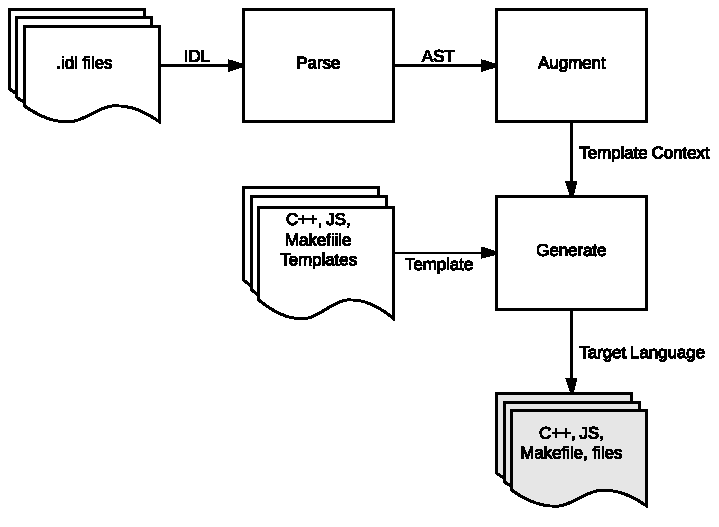
\includegraphics[width=0.9\textwidth]{generator.pdf} 
    \caption{Flow diagram showing the role of the generator}
    \label{fig:generator-diagram}
\end{figure}

We use the augmented AST as a \emph{context} to be passed to the template engine. We also add some helper functions on top of the template engine, to simplify the actual template. The template engine then uses the context to substitute the relevant strings into the correct places. For example, Listing \ref{code_template_context_eg} is a context that is used with the template shown in Listing \ref{code_template_eg} to generate the output shown in Listing \ref{code_template_output}. The rest of the code generator implementation is essentially augmenting the context to allow easy access for the template engine to generate all the files we needed.

Because the parser we used produces an AST in JavaScript, it made sense to have the generator in JavaScript too. This means we had to find a JavaScript template engine. There is more than a dozen template engine available to choose from, however, to simplify the templates and make them as human-readable as possible, we decided to limit our search only to templates with simple markup and logics. One template notation stood out, mustache\cite{mustache}. Mustache is an elegant, simple, templating language used across many languages. We decided to go with it because of its good documentation on its notation, its popularity, and its simplicity. However, several implementations of mustache existed. There was mustache.js\cite{mustachejs}, handlebars\cite{handlebarsjs}, and hogan\cite{hoganjs} by twitter. After considering each implementation, we found that they were very similar. We decided to choose hogan for its simplicity, speed, and extra features.

\lstset{language=C,caption={An example of a template context},label=code_template_context_eg}
\begin{code}
{
  timestamp: "Thu May 08 2014 21:38:16 GMT+0100 (BST)",
  moduleName: "Bullet",
  dictionaries: [{
    name: "XYZ",
    members: [
      { name: "x", STDTypeName: "float"},
      { name: "y", STDTypeName: "float"},
      { name: "z", STDTypeName: "float"}
    ]
  }]
}
\end{code}

\lstset{language=C,caption={An example of a template},label=code_template_eg}
\begin{code}
/* AUTOMATICALLY GENERATED ON {{timestamp}} */

#ifndef PPRPCGEN_{{moduleName}}_TYPES_H_
#define PPRPCGEN_{{moduleName}}_TYPES_H_

#include <string>
#include <vector>

namespace pprpcgen{
{{#dictionaries}}
typedef struct {
  {{#members}}
  {{^typeIsSequence}}{{STDTypeName}}{{/typeIsSequence}}
  {{#typeIsSequence}}std::vector<{{STDTypeName}}>{{/typeIsSequence}}
  {{name}};
  {{/members}}
} {{name}};

{{/dictionaries}}

}

#endif /* PPRPCGEN_{{moduleName}}_TYPES_H_ */

\end{code}

\lstset{language=C,caption={An example of the output of the generator},label=code_template_output}
\begin{code}
/* AUTOMATICALLY GENERATED ON Fri Jun 06 2014 20:11:41 GMT+0100 (BST) */

#ifndef PPRPCGEN_Bullet_TYPES_H_
#define PPRPCGEN_Bullet_TYPES_H_

#include <string>
#include <vector>

namespace pprpcgen{

typedef struct {
  float x;
  float y;
  float z;
} XYZ;

}

#endif /* PPRPCGEN_Bullet_TYPES_H_ */

\end{code}

% subsection code_generators_design (end)

% section generating_rpc_code (end)



\newpage